% ═══════════════════════════════════════════════════════════════════════════
%  DDF — préambule commun aux sept articles.  % ═══════════════════════════════════════════════════════════════════════════
%  DDF — préambule commun aux sept articles.  % ═══════════════════════════════════════════════════════════════════════════
%  DDF — préambule commun aux sept articles.  \input{ddf-common} en tête.
%  Définit : la mise en page, les macros, le bloc de série, la déclaration
%  d'usage d'outils, et le bloc de traçabilité.
% ═══════════════════════════════════════════════════════════════════════════
\documentclass[11pt,a4paper]{article}
\usepackage[margin=2.3cm]{geometry}
\usepackage{amsmath,amssymb,booktabs,hyperref,graphicx,xcolor}
\usepackage[expansion=false]{microtype}
\hypersetup{colorlinks=true,linkcolor=blue!45!black,citecolor=blue!45!black,urlcolor=blue!45!black}

% ---------- macros physiques ----------
\newcommand{\MPl}{M_{\rm Pl}}\newcommand{\Mred}{\bar M_{\rm Pl}}
\newcommand{\Mfive}{M_5}\newcommand{\MS}{M_S}\newcommand{\V}{\mathcal V}
\newcommand{\Neff}{N_{\rm eff}}\newcommand{\cb}{c_b}\newcommand{\ab}{\alpha_b}

% ---------- étiquettes épistémiques ----------
\newcommand{\Derived}{\textit{[Derived]}}
\newcommand{\Input}{\textit{[Input, natural]}}
\newcommand{\Posited}{\textit{[Posited]}}
\newcommand{\Candidate}{\textit{[Candidate]}}
\newcommand{\Open}{\textit{[Open, declared]}}
\newcommand{\Verified}{\textit{[Verified]}}

% ---------- bloc de série : \seriesdate{III}{The medium} ----------
\newcommand{\seriesdate}[2]{%
 \date{\small \textit{Cosmic Shadow Geometry} \\ \small Article #1 of VII
 \,\textperiodcentered\, #2 \,\textperiodcentered\, \today}}

% ---------- déclaration d'outils, identique dans les sept ----------
\newcommand{\toolsstatement}{%
\section*{Declaration on computational tools}
\addcontentsline{toc}{section}{Declaration on computational tools}
\small
This work was carried out by the author alone, without institutional affiliation.
\textbf{Large language models were used as computational and analytical assistants
throughout}: to write and debug the numerical scripts, to run the scans and
minimisations, to produce the figures, to check algebra and dimensional
consistency, to search and summarise the literature, and to audit drafts for
internal contradictions. Several distinct systems were used and cross-checked
against one another; no single system's output was accepted without an
independent numerical or analytical verification.

\textbf{The author is solely responsible for the physical hypotheses, the
interpretation of every result, the epistemic labels attached to each claim, and
the decision of what to publish and what to withdraw.} All quantitative
statements in this paper are reproduced by the scripts listed in the
traceability section; a reader who runs them obtains the numbers printed here
without needing any language model. Where an earlier draft contained an error
introduced by an unverified computation, it is recorded as a withdrawal rather
than silently removed.
\normalsize}

% ---------- bloc de traçabilité : \traceability{V}{...} ----------
\newcommand{\traceability}[2]{%
\section*{Data availability, traceability and reproducibility}
\addcontentsline{toc}{section}{Traceability}
\small
Every number, table and figure in this paper is regenerated by the scripts of
this article's folder. The complete repository ---sources, scripts, proof files,
figures and compiled documents for all seven articles--- is at
\url{https://github.com/HBoufourou}.

\textbf{Folder \texttt{article-#1/} contains:}
\begin{itemize}\itemsep2pt
\item \texttt{tex/} --- the \LaTeX\ source and the shared preamble \texttt{ddf-common.tex};
\item \texttt{scripts/} --- every computation, each runnable standalone with
      \texttt{python3 <name>.py} and printing its own verification verdict;
\item \texttt{proofs/} --- the JSON files carrying the certified values.
      \textbf{Any number absent from \texttt{proofs/} is not certified};
\item \texttt{data/} --- the CSV tables underlying the figures;
\item \texttt{figures/} --- the PNG files, regenerated by \texttt{scripts/figures.py};
\item \texttt{pdf/} --- the compiled article;
\item \texttt{VERIFICATION.txt} --- the output of the verification suite.
\end{itemize}
#2
\normalsize}
 en tête.
%  Définit : la mise en page, les macros, le bloc de série, la déclaration
%  d'usage d'outils, et le bloc de traçabilité.
% ═══════════════════════════════════════════════════════════════════════════
\documentclass[11pt,a4paper]{article}
\usepackage[margin=2.3cm]{geometry}
\usepackage{amsmath,amssymb,booktabs,hyperref,graphicx,xcolor}
\usepackage[expansion=false]{microtype}
\hypersetup{colorlinks=true,linkcolor=blue!45!black,citecolor=blue!45!black,urlcolor=blue!45!black}

% ---------- macros physiques ----------
\newcommand{\MPl}{M_{\rm Pl}}\newcommand{\Mred}{\bar M_{\rm Pl}}
\newcommand{\Mfive}{M_5}\newcommand{\MS}{M_S}\newcommand{\V}{\mathcal V}
\newcommand{\Neff}{N_{\rm eff}}\newcommand{\cb}{c_b}\newcommand{\ab}{\alpha_b}

% ---------- étiquettes épistémiques ----------
\newcommand{\Derived}{\textit{[Derived]}}
\newcommand{\Input}{\textit{[Input, natural]}}
\newcommand{\Posited}{\textit{[Posited]}}
\newcommand{\Candidate}{\textit{[Candidate]}}
\newcommand{\Open}{\textit{[Open, declared]}}
\newcommand{\Verified}{\textit{[Verified]}}

% ---------- bloc de série : \seriesdate{III}{The medium} ----------
\newcommand{\seriesdate}[2]{%
 \date{\small \textit{Cosmic Shadow Geometry} \\ \small Article #1 of VII
 \,\textperiodcentered\, #2 \,\textperiodcentered\, \today}}

% ---------- déclaration d'outils, identique dans les sept ----------
\newcommand{\toolsstatement}{%
\section*{Declaration on computational tools}
\addcontentsline{toc}{section}{Declaration on computational tools}
\small
This work was carried out by the author alone, without institutional affiliation.
\textbf{Large language models were used as computational and analytical assistants
throughout}: to write and debug the numerical scripts, to run the scans and
minimisations, to produce the figures, to check algebra and dimensional
consistency, to search and summarise the literature, and to audit drafts for
internal contradictions. Several distinct systems were used and cross-checked
against one another; no single system's output was accepted without an
independent numerical or analytical verification.

\textbf{The author is solely responsible for the physical hypotheses, the
interpretation of every result, the epistemic labels attached to each claim, and
the decision of what to publish and what to withdraw.} All quantitative
statements in this paper are reproduced by the scripts listed in the
traceability section; a reader who runs them obtains the numbers printed here
without needing any language model. Where an earlier draft contained an error
introduced by an unverified computation, it is recorded as a withdrawal rather
than silently removed.
\normalsize}

% ---------- bloc de traçabilité : \traceability{V}{...} ----------
\newcommand{\traceability}[2]{%
\section*{Data availability, traceability and reproducibility}
\addcontentsline{toc}{section}{Traceability}
\small
Every number, table and figure in this paper is regenerated by the scripts of
this article's folder. The complete repository ---sources, scripts, proof files,
figures and compiled documents for all seven articles--- is at
\url{https://github.com/HBoufourou}.

\textbf{Folder \texttt{article-#1/} contains:}
\begin{itemize}\itemsep2pt
\item \texttt{tex/} --- the \LaTeX\ source and the shared preamble \texttt{ddf-common.tex};
\item \texttt{scripts/} --- every computation, each runnable standalone with
      \texttt{python3 <name>.py} and printing its own verification verdict;
\item \texttt{proofs/} --- the JSON files carrying the certified values.
      \textbf{Any number absent from \texttt{proofs/} is not certified};
\item \texttt{data/} --- the CSV tables underlying the figures;
\item \texttt{figures/} --- the PNG files, regenerated by \texttt{scripts/figures.py};
\item \texttt{pdf/} --- the compiled article;
\item \texttt{VERIFICATION.txt} --- the output of the verification suite.
\end{itemize}
#2
\normalsize}
 en tête.
%  Définit : la mise en page, les macros, le bloc de série, la déclaration
%  d'usage d'outils, et le bloc de traçabilité.
% ═══════════════════════════════════════════════════════════════════════════
\documentclass[11pt,a4paper]{article}
\usepackage[margin=2.3cm]{geometry}
\usepackage{amsmath,amssymb,booktabs,hyperref,graphicx,xcolor}
\usepackage[expansion=false]{microtype}
\hypersetup{colorlinks=true,linkcolor=blue!45!black,citecolor=blue!45!black,urlcolor=blue!45!black}

% ---------- macros physiques ----------
\newcommand{\MPl}{M_{\rm Pl}}\newcommand{\Mred}{\bar M_{\rm Pl}}
\newcommand{\Mfive}{M_5}\newcommand{\MS}{M_S}\newcommand{\V}{\mathcal V}
\newcommand{\Neff}{N_{\rm eff}}\newcommand{\cb}{c_b}\newcommand{\ab}{\alpha_b}

% ---------- étiquettes épistémiques ----------
\newcommand{\Derived}{\textit{[Derived]}}
\newcommand{\Input}{\textit{[Input, natural]}}
\newcommand{\Posited}{\textit{[Posited]}}
\newcommand{\Candidate}{\textit{[Candidate]}}
\newcommand{\Open}{\textit{[Open, declared]}}
\newcommand{\Verified}{\textit{[Verified]}}

% ---------- bloc de série : \seriesdate{III}{The medium} ----------
\newcommand{\seriesdate}[2]{%
 \date{\small \textit{Cosmic Shadow Geometry} \\ \small Article #1 of VII
 \,\textperiodcentered\, #2 \,\textperiodcentered\, \today}}

% ---------- déclaration d'outils, identique dans les sept ----------
\newcommand{\toolsstatement}{%
\section*{Declaration on computational tools}
\addcontentsline{toc}{section}{Declaration on computational tools}
\small
This work was carried out by the author alone, without institutional affiliation.
\textbf{Large language models were used as computational and analytical assistants
throughout}: to write and debug the numerical scripts, to run the scans and
minimisations, to produce the figures, to check algebra and dimensional
consistency, to search and summarise the literature, and to audit drafts for
internal contradictions. Several distinct systems were used and cross-checked
against one another; no single system's output was accepted without an
independent numerical or analytical verification.

\textbf{The author is solely responsible for the physical hypotheses, the
interpretation of every result, the epistemic labels attached to each claim, and
the decision of what to publish and what to withdraw.} All quantitative
statements in this paper are reproduced by the scripts listed in the
traceability section; a reader who runs them obtains the numbers printed here
without needing any language model. Where an earlier draft contained an error
introduced by an unverified computation, it is recorded as a withdrawal rather
than silently removed.
\normalsize}

% ---------- bloc de traçabilité : \traceability{V}{...} ----------
\newcommand{\traceability}[2]{%
\section*{Data availability, traceability and reproducibility}
\addcontentsline{toc}{section}{Traceability}
\small
Every number, table and figure in this paper is regenerated by the scripts of
this article's folder. The complete repository ---sources, scripts, proof files,
figures and compiled documents for all seven articles--- is at
\url{https://github.com/HBoufourou}.

\textbf{Folder \texttt{article-#1/} contains:}
\begin{itemize}\itemsep2pt
\item \texttt{tex/} --- the \LaTeX\ source and the shared preamble \texttt{ddf-common.tex};
\item \texttt{scripts/} --- every computation, each runnable standalone with
      \texttt{python3 <name>.py} and printing its own verification verdict;
\item \texttt{proofs/} --- the JSON files carrying the certified values.
      \textbf{Any number absent from \texttt{proofs/} is not certified};
\item \texttt{data/} --- the CSV tables underlying the figures;
\item \texttt{figures/} --- the PNG files, regenerated by \texttt{scripts/figures.py};
\item \texttt{pdf/} --- the compiled article;
\item \texttt{VERIFICATION.txt} --- the output of the verification suite.
\end{itemize}
#2
\normalsize}

\graphicspath{{figures/}{../figures/}}
\title{\textbf{The Dark Dimension Framework IV:\\ One scale and its shadow --- the structure of the framework}}
\author{Hicham Boufourou\\ \small\textit{Independent Researcher, Brussels, Belgium}\\ \small\texttt{hicham.boufourou@hotmail.com}}
\seriesdate{IV}{One scale and its shadow}
\begin{document}\maketitle
\begin{abstract}
\noindent The first three articles built a geometry, derived a tower, and let a medium act. This closing article steps back and states what the framework \emph{is}. Its starting point is a structural fact established in Article II: the millielectronvolt sector is not several coincidences but one --- the triplet $(\ell,\varepsilon,u)$ closes on the single knot $m_{\Phi}=\varepsilon\approx1/R=24$~meV. The candidate explanation is the oldest mechanism in the supersymmetric literature, read in a new place: gravity-mediated transmission, $\mu=\MS^{2}/\MPl$, under which the entire meV sector is the \emph{gravitational shadow} of one TeV scale on the wall. The lineage is declared before the construction: the relation is that of Dimopoulos--Giudice (1996) and of the gravitino; the identification of a micron dark dimension with fundamental scales is the dark-dimension programme of Montero, Vafa and Valenzuela; and the specific bridge --- supersymmetry breaking at $\mathcal{O}$(TeV) tied to a meV bulk --- is the swampland statement of Anchordoqui, Antoniadis, Cribiori, L\"ust and Scalisi. This framework does not rediscover the relation; it \emph{joins} that ecosystem through its supersymmetric door and adds its own instruments: three new members of the convergence, a testable ratio structure, and an experimental triangle. The companion article reads the same relation from the ultraviolet side, where a meV sector generated by $\mu=\MS^{2}/\MPl$ is the moduli spectrum of a compactification with supersymmetry broken at the TeV; that reading is a consistency check between two descriptions, not a derivation of either, and it is confined to Appendix~C. Numerically, $\mu=24.1$~meV at $\MS=7.6$~TeV, and six independently obtained quantities --- the wall tension inverted from the derived well ($9.8$~TeV), the localisation thickness, the radion stiffness, the nucleation scale, the collider-compatible supersymmetry band, and the meV knot lifted by $\sqrt{(1/R)\MPl}$ --- land in one band, $\sim$4--10~TeV. Every bulk mass is then $c_{i}\times\mu$ with $c_{i}$ of order unity: the tower anchors the spectrum at $c=1$; the radion window of Article I, an honest order estimate there, is here \emph{explained} as $c_{r}\in[0.21,1.7]$; the source field sits below $0.18$; and the gravitino of the inherited scenario imports at $13.9$~meV. The statement is falsifiable in one sentence: every bulk mass of this framework lies within one decade of $\mu$ --- a single state found at the eV or the $\mu$eV kills the structure whole. An internal cross-check closes the accounting: $\Lambda^{1/4}/\mu=0.093\approx1/4\pi$, so the hierarchy between the dark-energy scale and the sector scale is a loop factor, not a new scale --- below $\MS$ the framework contains no free scale at all. The experimental consequence is a triangle: the torsion balance reads the radion window, which \emph{is} a window on $\MS$ (3.5--9.8~TeV); a next-generation collider reads $\MS$ directly; and LISA reads the transition dynamics at the same scale. Two instruments that have never shared a parameter would be measuring the same number from two ends, with a third to arbitrate. The article ends with the complete map of the framework --- what is derived, what is candidate, what is input and natural, what is measured, what only data can decide, and what is inherited from the cosmological constant --- and with the compiled list of everything that kills it.
\end{abstract}

\section{The knot}
Article II left the meV sector in an unusual condition for a dark-sector model: over-determined. The well slope, the level unit, the mode length and the interval closed into the triplet $(\ell,\varepsilon,u)=(5.81~\mu\mathrm{m},\,24~\mathrm{meV},\,4.43)$ with the single identification
\begin{equation}
m_{\Phi}\;=\;\varepsilon\;\approx\;\frac{1}{R}\;=\;24~\mathrm{meV}.
\label{eq:knot}
\end{equation}
What early statements of this framework treated as a cluster of coincidences --- the tower scale near the dark-energy scale, the mass near the inverse radius, the slope's square root near both --- is one statement, Eq.~(\ref{eq:knot}), made once. A single knot demands a single explanation, and the shape of Eq.~(\ref{eq:knot}) itself points at it: a millielectronvolt is what the Planck mass makes of a TeV,
\begin{equation}
\frac{(\mathrm{TeV})^{2}}{\MPl}\;\sim\;\mathrm{meV}.
\end{equation}
The rest of this article takes that arithmetic seriously, declares whose it is, and asks what it predicts. [Knot: Derived (Article II); its explanation below: Candidate] This framework is a dark dimension in the sense of Montero, Vafa and Valenzuela; the name records its central structure, the shadow relation of Article~IV, under which the entire millielectronvolt sector is the gravitational shadow of one TeV scale. A fifth article, cited throughout as the \emph{companion}, examines whether this geometry admits an ultraviolet completion in Type~I$'$ string theory; it is a companion, not a foundation, and nothing in Articles~I--IV depends on it.

\section{Standing on shoulders: the shadow relation and its lineage}
The rule of this series is that provenance is stated before construction. The relation
\begin{equation}
\mu\;=\;\frac{\MS^{2}}{\MPl}
\label{eq:shadow}
\end{equation}
--- a heavy scale $\MS$ casting a light gravitational shadow $\mu$ --- is the founding arithmetic of gravity-mediated supersymmetry breaking: it is the gravitino mass relation, and its phenomenological reading, that TeV-scale breaking implies new gravitational-strength physics at sub-millimetre range, is Dimopoulos and Giudice (1996) \cite{DG96}, extended into the weak-scale compactification programme of Antoniadis, Arkani-Hamed, Dimopoulos and Dvali \cite{ADD98}. The identification of a single micron-scale dark dimension as a fundamental feature tied to the cosmological constant is the dark-dimension scenario of Montero, Vafa and Valenzuela \cite{MVV}; and the specific bridge used here --- supersymmetry broken at $\mathcal{O}$(TeV), tied by the gravitino constraint to the meV bulk, ``within reach of the LHC'' --- is the statement of Anchordoqui, Antoniadis, Cribiori, L\"ust and Scalisi \cite{AAL}, with the astrophysics of a meV gravitino developed by Law-Smith, Obied, Prabhu and Vafa \cite{CPV}. This framework therefore claims no discovery in Eq.~(\ref{eq:shadow}), and it is important to be precise about what it does and does not bring. The relation is inherited whole from the gravity-mediated literature; it is not re-derived here, and no attempt is made to dress an inheritance as a derivation. What the framework brings is a \emph{junction}, and the junction has content: built upward from galactic phenomenology and laboratory windows --- the derived well of Article II, the closed amplitude, the measured switch of Article III --- the Dark Dimension Framework arrives, by its own route and without Eq.~(\ref{eq:shadow}) in hand, at a TeV--meV coincidence that the relation then organises. The junction is not asserted: it is tested by the six-fold convergence of \S3, in which six independently obtained TeV quantities of this series land in one band, and by the experimental triangle of \S6, which the top-down programme does not possess. The relation is the oldest mechanism in the supersymmetric literature; the test structure built on it here is new. [Positioning: declared; the claim class is synthesis with testable content, not derivation of the relation]

An honest objection must be met here rather than left to the reader: if the relation is inherited, has anything been derived? The answer is that the derivation programme of this series produced its own content independently of Eq.~(\ref{eq:shadow}) --- the well twice, the closed amplitude, the two dials, the universal response, the decoherence threshold, the confirmed wide-binary null --- and that the relation then organises the one coincidence those derivations left standing, the knot of Article II. The relation is the explanation of the knot; the knot, and everything else in the series, was derived without it. If the relation fails, the framework degrades gracefully --- this article dies, Articles I--III stand as an unexplained but functioning machine; if it holds, the coincidence becomes an identity. Neither outcome requires the framework to have derived the relation itself.

\section{The six-fold convergence}
Read Eq.~(\ref{eq:shadow}) in both directions. Downward: a wall-scale $\MS$ in the collider-adjacent band gives $\mu=\MS^{2}/\MPl$ of $5.1$, $8.8$, $24.1$ and $40.0$~meV at $\MS=3.5$, $4.6$, $7.6$ and $9.8$~TeV. Upward: the knot lifts to
\begin{equation}
\sqrt{(1/R)\,\MPl}\;=\;7.6~\mathrm{TeV},
\end{equation}
and the radion window of Article I, 5--40~meV, lifts to $\MS\in3.5$--$9.8$~TeV. Now place beside these every TeV-scale quantity this series has produced, each obtained independently and none with Eq.~(\ref{eq:shadow}) in hand:
\begin{center}\small
\begin{tabular}{llll}
\toprule
\textbf{Quantity} & \textbf{Value} & \textbf{Origin} & \textbf{Article}\\
\midrule
Wall tension $T^{1/4}$ & $9.8$~TeV (window 2--13) & inversion of the derived well & II \S2.1\\
Localisation $L_{g}^{-1}$ & 1--10~TeV & thin-core one-scale wall & I \S3\\
Radion stiffness $V_{\rm stab}^{1/4}$ & 3.5--10~TeV & $\sqrt{m_{r}\MPl}$ over the window & I \S5\\
Nucleation scale & $\sim$6~TeV & bounce action $S_{3}/T\simeq140$ & dossier\\
Supersymmetry band & 4--10~TeV & collider floor $+$ budgets & dossier\\
meV knot, lifted & $7.6$~TeV & $\sqrt{(1/R)\MPl}$ & this article\\
\bottomrule
\end{tabular}
\end{center}
Six quantities, six origins, one band --- and the sharpest pair is the most telling: the tension inverted from the well ($9.8$~TeV, Article II) and the knot lifted by the shadow ($7.6$~TeV) agree to within thirty percent, with no common input between them --- the precision that the declared order-one coefficients (the $1/6$ of the gravitational slope, the $\mathcal{O}(1)$ of the shadow relation) actually allow, and no better agreement should be claimed. Under Eq.~(\ref{eq:shadow}) the coincidence is not arranged, it is an identity: the same wall that binds the tower gravitationally \emph{is} the scale whose shadow sets the tower's mass. The two-origins structure that Article II established honestly --- a TeV core and a meV source sector, dynamically independent --- is here not repaired but explained: they are independent the way an object and its shadow are, connected only through $1/\MPl$. [Candidate, order of magnitude; convergence: computed]

\begin{figure}[t]
\centering
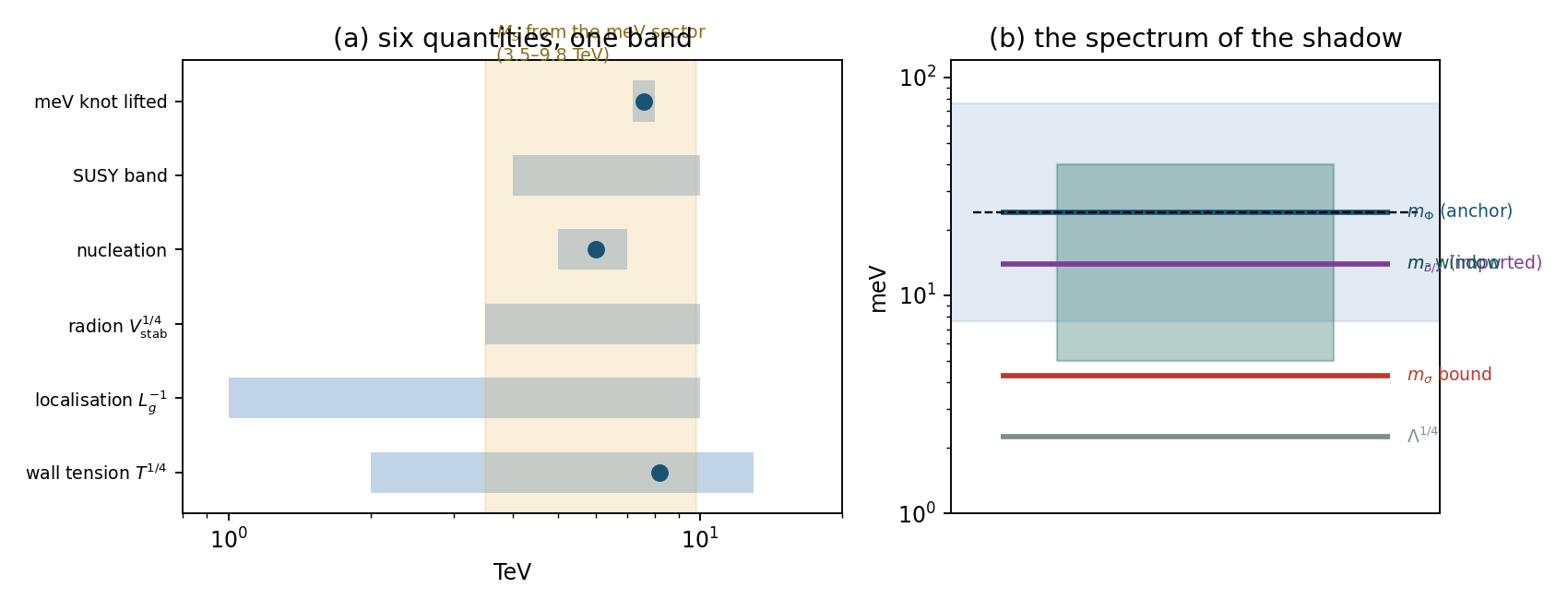
\includegraphics[width=0.95\textwidth]{fig1_convergence.png}
\caption{The six-fold convergence. Left: the six independently obtained TeV quantities of the series (bars: windows; markers: central values) against the band $\MS=3.5$--$9.8$~TeV implied by the meV sector under $\mu=\MS^{2}/\MPl$. Right: the shadow arithmetic --- one wall scale, transmitted by $1/\MPl$, lands on the knot of Article II. [\texttt{shadow.py}]}
\label{fig:conv}
\end{figure}

The convergence of this section is not a prediction of Eq.~(\ref{eq:shadow}); it is the \emph{evidence} for it. Six TeV quantities, each obtained independently of the relation and of each other, land in the band the relation implies from the meV knot; were it false, the agreement of the sharpest pair --- the tension inverted from the well and the knot lifted by the shadow, thirty percent apart with no common input --- would be a numerical accident with no organising principle. That is what licenses the [Candidate] label: a structural relation supported at order of magnitude, not yet a derivation, and labelled as such. The convergence is built from six quantities of this series alone; the gravitino of the inherited scenario, adopted in \S4, plays no role in it.

\section{The spectrum of the shadow}
If the meV sector is a shadow, every bulk mass should be an order-one coefficient times the one shadow scale, $m_{i}=c_{i}\,\mu$ with $\mu=24.1$~meV at the anchor. The series' inventory reads:
\begin{center}\small
\begin{tabular}{lllll}
\toprule
\textbf{State} & \textbf{Framework value} & $c_{i}$ & \textbf{Status} & \textbf{Provenance}\\
\midrule
Tower / bulk field $m_{\Phi}$ & 24~meV & $1.0$ & the anchor (Eq.~\ref{eq:knot}) & Derived (Art.~II)\\
Radion $m_{r}$ & 5--40~meV window & $0.21$--$1.7$ & the window \emph{explained} & Window (Art.~I)\\
Source field $m_{\sigma}$ & $<4.3$~meV (dial, Art.~II) & $<0.18$ & bounded, order consistent & Bound (Art.~II)\\
Gravitino $m_{3/2}$ & $\mu/\sqrt{3}=13.9$~meV & $0.58$ & adopted, not derived & Imported \cite{AAL,CPV}\\
\bottomrule
\end{tabular}
\end{center}
Article I called the radion mass an order estimate and drew a window; this table is the window's explanation --- $c_{r}$ of order unity is exactly what a shadow spectrum gives, and the honesty of Article I converts here into structure. The gravitino line is adopted, not derived. It is imported from the inherited supersymmetric scenario \cite{AAL,CPV}, where the meV gravitino is the dark dimension's companion and its astrophysical viability is analysed in \cite{CPV}. The framework adopts the entry with its provenance visible, but the gravitino does not count among its own productions: it is a guest in the spectrum, not a resident. If the supersymmetric scenario is not realised, the gravitino line simply leaves the table, and the convergence, the spectrum rule $c_{i}\mu$ for the remaining states, and the one-decade statement all stand unchanged. The falsifiable statement is one sentence: \textbf{every bulk mass of this framework lies within one decade of $\mu$}. A dark-sector state established at the eV, or at the $\mu$eV, does not wound the structure --- it kills it whole, anchor and shadow together. The $c_{i}$ themselves are ultraviolet numbers, in the same class as $c_{b}$ (Article I): order unity by construction, not derivable at the effective level, and declared so. [Candidate spectrum; one-decade statement: the article's own executioner]

\section{The loop cross-check}
One scale remains unaccounted: the dark-energy density itself, $\Lambda^{1/4}=2.25$~meV, an order below the sector scale. Form the ratio:
\begin{equation}
\frac{\Lambda^{1/4}}{\mu}\;=\;\frac{2.25}{24.1}\;=\;0.093\;\approx\;\frac{1}{4\pi}\;=\;0.080 .
\end{equation}
The hierarchy \emph{inside} the meV sector is a loop factor --- the most ordinary suppression quantum field theory owns --- and not a new scale. The accounting below $\MS$ then closes completely: one shadow scale $\mu$, order-one coefficients $c_{i}$, and a one-loop step down to $\Lambda^{1/4}$; \textbf{no free scale exists in this framework between the wall and the vacuum}. The statement is a consistency at order of magnitude, labelled as such --- it does not derive the value of $\Lambda$ (nothing in this series does; that is the S-3 class, inherited and declared in Article I) --- but it is the difference between a sector with a spectrum and a sector with a story. [Candidate, order of magnitude]

One honesty must be renewed here rather than quietly absorbed, and the renewal must be explicit because the shadow relation is the framework's prettiest structure, and the temptation to let it launder the framework's debts is real. The shadow does not absolve the source tadpole. Article II declared the capacitor's coupling tension --- $g\gtrsim2\times10^{3}\sqrt{\Mfive}$ from the $\Lambda$ budget --- and showed it immune to 't~Hooft protection at the fundamental cutoff (fifty-one orders) \emph{and} to TeV supersymmetry (forty-one orders at the $\MS$ cutoff: protecting a meV tadpole would need supersymmetry down to the meV, which nothing here provides). The shadow relation organises the sector's \emph{masses}; it does not soften that one coupling: the six-fold convergence of \S3 is built from the TeV quantities of the series, none of which involves the tadpole's naturalness --- the convergence stands independently of the tension, and the tension independently of the convergence. A framework that let its prettiest structure launder its declared debts would not deserve the map of \S7, and this framework does not. The tension remains exactly where Article II filed it --- the cosmological-constant class --- and it will remain there until the cosmological-constant problem itself moves. [S-3, renewed]

\section{The experimental triangle}
The structure pays its way in instruments. Because the radion window \emph{is} a window on $\MS$ under Eq.~(\ref{eq:shadow}), three unrelated machines become three reads of one number. \emph{The balance:} the torsion-balance campaign of Article I, scanning 5--40~$\mu$m, reads $m_{r}$ --- and thereby $\MS=\sqrt{m_{r}\MPl}$ to the width of $c_{r}$: a fifth-force laboratory measuring the supersymmetry-breaking scale. \emph{The collider:} a machine reaching the 4--10~TeV band reads $\MS$ directly; the inherited scenario's own phrasing --- within reach of the next generation --- applies verbatim, and agreement or disagreement with the balance's inference is a clean structural test. \emph{The interferometer:} if the wall's transition is first order, its bubble dynamics at $\MS$ radiate a stochastic background in the LISA band with $\beta/H\in[10,100]$ --- conditional on first-orderness, which the framework does not derive, and declared so; the gravitational-wave read closes the triangle. Two instruments that have never shared a parameter --- a table-top pendulum and a hundred-kilometre collider --- would be measuring the same quantity from two ends, with a million-kilometre interferometer to arbitrate. The framework does not merely tolerate the coming decade of experiments; it is \emph{about} them. [Derived consequence of the Candidate; $\beta/H$ conditional]

\begin{figure}[t]
\centering

\includegraphics[width=0.9\textwidth]{fig2_spectrum_triangle.png}
\caption{Left: the spectrum of the shadow --- every bulk state at $c_{i}\times\mu$, all inside one decade (band); the one-decade statement is the structure's executioner. Right: the experimental triangle --- balance, collider and interferometer as three reads of the single scale $\MS$. [\texttt{shadow.py}]}
\label{fig:spec}
\end{figure}

\section{The map of the framework}
This series set out to state a theory that knows what it knows. The full inventory:

\emph{Derived.} The volume dilution and $\Mfive$; the $8/3$ short-range law; the one-scale wall $T^{1/4}=L_{g}^{-1}$; the covariant vertex and $\alpha_{b}=c_{b}\sqrt{2w_{1}}$; the linear well, twice, and the tension inversion $T^{1/4}=9.8$~TeV; the interleaved tower and its ratios; $u=4.43$ and the closed triplet; the two dials; $w_{1}=5.5$ and the closed amplitude; the drip's suppression and stimulation; the $\lambda$ window's two jaws; the response law with one $g_{\dagger}$; the decoherence form with one $K$; the Solar-System bubble and Cassini met identically; the cluster mass budget; the radion's double no-go and $|1+w|$; the budgets of Article I.

\emph{Candidate (order of magnitude, mechanism posited).} The shadow relation as the knot's explanation; the six-fold convergence as identity; the spectrum $c_{i}\mu$; the loop step to $\Lambda^{1/4}$.

\emph{Input, natural (ultraviolet numbers, declared).} $c_{b}$; the $c_{i}$; the wall's single scale within its band.

\emph{Posited (choices, labelled).} The misalignment fractions (no Airy identity fixes them); the gauge-localisation mechanism; the cluster tier-two scaling (conclusion insensitive).

\emph{Measured (by this series or its companions).} $f\in[1.2\times10^{-3},8.42\times10^{-3}]$; the universality bound $|\Delta\alpha_{b}/\alpha_{b}|\leq9$--$14\%$; the wide-binary null $\gamma=1.00$--$1.05$ as confirmed prediction.

\emph{Data-driven (pre-registered triggers, waiting).} The balance at $8.2~\mu$m and the window scan; the tower dials; Gaia DR4 and the mobile-cutoff test\footnote{The mobile cutoff is the per-pair decoherence radius $s_{c}\propto M^{1/3}$ of Article~III: pairs are compared inside versus beyond their own $s_{c}$, and the mass-binned ratio is free of $f$, $\rho$ and $K$. The full pre-registered protocol (blinding scheme, thresholds) is archived and timestamped separately, ahead of the DR4 release.}; LISA; an independent $\Upsilon_{\star}$; the collider band.

\emph{S-3 (inherited, declared, not claimed solved).} The value of $\Lambda$; the depth of $V_{\rm stab}$ against the residual vacuum; the source tadpole's naturalness (shown immune to both 't~Hooft protection and TeV supersymmetry).

\emph{How the four articles interlock.} Article I is load-bearing for all: its calibration fixes $R$ and $\Mfive$, its vertex the coupling form, its budgets the cosmology's room. Article II consumes I's stage and produces the objects --- well, tower, $u$, $w_{1}$ --- that III's phenomenology spends; III consumes the amplitude and returns the measurements ($f$, the universality bound, the confirmed null) that close the loop back on II's dials. This article consumes all three and adds no object at all: only the relation among their scales, which is why it is last, and why killing any one of I--III kills IV for free while the converse is not true --- the shadow can die (a state outside the decade) leaving I--III standing as an unexplained but functioning machine. The series degrades gracefully, and in one direction.

Nothing in the framework lives outside this table. That --- more than any single number --- is what these four articles set out to build. [The map]

\section{How the whole framework dies}
Compiled from the series, in rough order of arrival. (1) \emph{The balance misses:} Newton at $8/3$, $8.2~\mu$m --- Article I dies, and the series with it; no parameter moves. (2) \emph{The window closes empty:} 5--40~$\mu$m scanned without a radion --- the stabilised geometry and the shadow's second line die together. (3) \emph{A state outside the decade:} any bulk mass at the eV or $\mu$eV --- Article IV dies whole. (4) \emph{The tower misbehaves:} non-$\sinh$ anharmonicity, or ratios homeless in $(m_{\sigma},u)$ --- Article II dies. (5) \emph{The switch fails:} DR4 wide binaries off Newton beyond the bubble, or a boost inside one --- Article III dies by its own pre-registered test. (6) \emph{The Bullet tightens} past the stimulated floor --- the drip stops. (7) \emph{Universality breaks} above $\sim$1\% with an independent $\Upsilon_{\star}$ --- the covariant vertex dies. (8) \emph{The collider band empties} while the balance finds the radion --- the triangle's two ends disagree, and the shadow was a shadow of nothing. (9) \emph{The source tadpole:} if a mechanism is found that generates the well slope without the super-natural coupling $g\gtrsim2\times10^{3}\sqrt{\Mfive}$, the capacitor's tension dissolves and the framework's most severe debt is paid; if instead the tension is shown unavoidable in any completion, the well's origin remains the framework's deepest open question --- a debt of the cosmological-constant class, not a flaw in the derivation. The framework stands, today, with every one of these executions scheduled and none delivered. It asks for nothing further from theory; the rest belongs to the sky, the bench, and the ring.

\appendix
\section{The derivation programme behind this series}
The final series condenses an audited derivation programme whose full traceability accompanies the dossiers; its verdicts, positive and negative alike, are what license the labels used above. \emph{The well:} a first thesis (a single wall-soliton doing double duty) was refuted by its own pre-registered criterion --- a 174~$\mu$m kink cannot inhabit a 25.8~$\mu$m corridor --- and corrected into the capacitor of Article II; the hoped-for structural link between the well slope and the radion stiffness was then refuted honestly (the capacitor's contribution to the radion mass falls twenty-eight orders short), establishing the two-origins structure that \S3 explains rather than repairs. \emph{The knot:} the interval-to-well ratio, once read off the spectrum, was computed and found exact ($u=4.43$), collapsing the sector's coincidences into Eq.~(\ref{eq:knot}). \emph{The self-sourced alternative:} the elegant possibility that the tower digs its own well ($J_{0}\propto\langle\Phi^{2}\rangle$) was constructed and killed on two counts --- the fixed point demands a coupling twelve orders beyond natural, and it would make the well track local density, breaking the universal tower --- so the coincidence it hoped to explain passed instead to the shadow relation of this article. \emph{The tadpole:} interrogated three ways and filed as S-3 (\S5). \emph{Universality:} converted from assumption to measurement (Article III \S7). The programme closed when every remaining open point was either a pre-registered data trigger, an ultraviolet number declared as input, or the inherited S-3 class --- the state this article maps. Negative results are listed with the same care as positive ones because they are load-bearing: each dead branch is a reason the surviving structure has the shape it has.


% ═══════════════════════════════════════════════════════════════════════════
%  APPENDICE DE LIAISON — identique dans les sept articles.
%  % ═══════════════════════════════════════════════════════════════════════════
%  APPENDICE DE LIAISON — identique dans les sept articles.
%  % ═══════════════════════════════════════════════════════════════════════════
%  APPENDICE DE LIAISON — identique dans les sept articles.
%  \input{appendix-where} juste avant \begin{thebibliography} ou la biblio.
%  Il répond à : qui vit où, et qu'est-ce que la série a changé en cours de route.
% ═══════════════════════════════════════════════════════════════════════════
\section*{Appendix: which sector lives where, and what changed}
\addcontentsline{toc}{section}{Appendix: which sector lives where}

The series was written over several months and \textbf{two of its assignments moved}.
A reader who meets the articles out of order is owed an explicit map rather than an
inference, so it is given here, identically in all seven papers.

\subsection*{A.1 The three locations}
The geometry has three places where physics can sit: the \emph{brane} at $y=0$,
the \emph{bulk} of the $8.2\,\mu$m interval, and the \emph{far wall} at $y=\pi R$.
\begin{center}\small
\begin{tabular}{llll}\toprule
sector & lives on & carried by & established in\\\midrule
ordinary matter & \textbf{brane} & thin core, Standard Model & I\\
gravity, radion, graviton & \textbf{bulk} & five-dimensional fields & I\\
the mediator $\Phi$ and its tower & \textbf{bulk} & Airy states of the $|y|$ well & II\\
the galactic response & \textbf{bulk} $\to$ brane & $\Phi$ exchange between baryons & III\\
dark matter & \textbf{see A.2} & --- & III, revisited in VI\\
dark energy & \textbf{see A.3} & --- & III, revisited in VI\\
hidden gauge sector & \textbf{far wall} & eight D8 and one O8 & V\\\bottomrule
\end{tabular}
\end{center}

\subsection*{A.2 Dark matter: the reservoir, and what the wall reading adds}
Articles~I--IV place dark matter in the \emph{bulk}: the excited states of the Airy
tower, populated cold at birth, collisionless, carrying at least $98.6\%$ of the dark
sector's density. That assignment does the work in three places. It makes structure
formation identical to cold dark matter at linear order. It answers the Bullet Cluster
by mass budget alone --- cluster masses are cluster masses, and the lensing tracks the
reservoir, which is why the lensing--dynamics difficulty of purely modified dynamics is
not inherited. And it fixes the radiation budget of Article~I.

Article~VI proposes a different reading: dark matter as the ordinary matter of the six
other regions of the same wall, seen through the bulk, giving
$\Omega_{\rm DM}/\Omega_b=N_{\rm regions}-1=6$ against an observed $5.31$.
\textbf{These are not the same statement, and we do not pretend otherwise.}

What they share is everything the phenomenology uses: in both readings the dark
component is cold, collisionless, and carries the mass, so lensing, the Bullet Cluster
and linear structure formation are unaffected. What differs is the \emph{constituent}:
quanta of $\Phi$ in the first, baryons of other regions in the second.
\textbf{The two are compatible if the tower reservoir is not required to be the whole
of the dark matter} --- and Article~III's own argument only requires it to dominate the
budget, not to be exhaustive. \Open

\subsection*{A.3 Dark energy: a bulk scalar, then a brane curvature}
Articles~I--IV treat $\Phi$ as the dark-energy candidate --- a bulk scalar engine. That
attempt \emph{failed by forty orders of magnitude}: a four-dimensional scalar cannot
reach $2.4$~meV from a $10^{-13}$~eV engine scale. The failure is recorded, not hidden.

Article~VI relocates dark energy \emph{to the brane}, as the extrinsic curvature of the
D8 wall in the cosmological bulk, $\Lambda_4=\varepsilon^2(1/R)^4$ with
$\varepsilon\simeq10^{-2}$. The mechanism supplies $(1/R)^4$ outright and leaves a gap
of $10^4$ rather than $10^{40}$. \textbf{$\Phi$ is correspondingly demoted from
dark-energy candidate to dark-sector mediator}, which is the role Articles~II and III
already gave it in every equation they actually use. \Candidate, declared tuning.

\subsection*{A.4 The radial acceleration relation, and what makes galaxies turn}
The relation is the one place where brane and bulk are \emph{both} indispensable, and
where nothing has moved since Article~III.

Baryons sit on the brane. They source $\Phi$, which propagates in the bulk with mass
$m_\Phi=24$~meV and hence Compton range $8.2\,\mu$m --- microscopic, so no fifth force
acts between laboratory bodies. What acts at galactic scale is not the free field but
the \emph{medium}: the coherent component of the dark sector responds to the baryonic
distribution, and that response, read back on the brane, is the extra acceleration.
The response saturates, which is why it produces a relation --- an acceleration scale
$g_\dagger$ --- rather than a rescaling of Newton's constant.

Three consequences, all in Article~III and unchanged:
\begin{itemize}\itemsep2pt
\item the response couples to the trace $T^\mu_{\ \mu}$, hence to mass and not to
      composition; the universality is bounded on 171 SPARC galaxies;
\item the response is carried by at most $1.4\%$ of the dark sector, the coherent part,
      so it never competes with the reservoir in the mass budget --- \textbf{galaxies
      turn because of the medium, they weigh because of the reservoir};
\item the response \emph{dies} in weak field, which is the ultra-diffuse galaxy test,
      and it dies in a decoherence bubble around the Sun, which is why Cassini is
      satisfied identically rather than by tuning.
\end{itemize}
\textbf{Neither relocation of A.2 or A.3 touches this.} The galactic response was never
assigned to the dark-energy sector, and it is not the reservoir either; it is the third
role, and it is the one the framework was built to explain.

\subsection*{A.5 What a reader should carry between articles}
Articles~I--IV stand on their own evidence and are not modified by V--VII: no result of
theirs is derived from the string embedding, and the embedding cannot promote any of
their labels. What V--VII add is an ultraviolet origin for one constant, a candidate
geometry, and two consequences of that geometry. What they \emph{change} is recorded
above and nowhere else: two relocations, both declared, neither retroactive.
 juste avant \begin{thebibliography} ou la biblio.
%  Il répond à : qui vit où, et qu'est-ce que la série a changé en cours de route.
% ═══════════════════════════════════════════════════════════════════════════
\section*{Appendix: which sector lives where, and what changed}
\addcontentsline{toc}{section}{Appendix: which sector lives where}

The series was written over several months and \textbf{two of its assignments moved}.
A reader who meets the articles out of order is owed an explicit map rather than an
inference, so it is given here, identically in all seven papers.

\subsection*{A.1 The three locations}
The geometry has three places where physics can sit: the \emph{brane} at $y=0$,
the \emph{bulk} of the $8.2\,\mu$m interval, and the \emph{far wall} at $y=\pi R$.
\begin{center}\small
\begin{tabular}{llll}\toprule
sector & lives on & carried by & established in\\\midrule
ordinary matter & \textbf{brane} & thin core, Standard Model & I\\
gravity, radion, graviton & \textbf{bulk} & five-dimensional fields & I\\
the mediator $\Phi$ and its tower & \textbf{bulk} & Airy states of the $|y|$ well & II\\
the galactic response & \textbf{bulk} $\to$ brane & $\Phi$ exchange between baryons & III\\
dark matter & \textbf{see A.2} & --- & III, revisited in VI\\
dark energy & \textbf{see A.3} & --- & III, revisited in VI\\
hidden gauge sector & \textbf{far wall} & eight D8 and one O8 & V\\\bottomrule
\end{tabular}
\end{center}

\subsection*{A.2 Dark matter: the reservoir, and what the wall reading adds}
Articles~I--IV place dark matter in the \emph{bulk}: the excited states of the Airy
tower, populated cold at birth, collisionless, carrying at least $98.6\%$ of the dark
sector's density. That assignment does the work in three places. It makes structure
formation identical to cold dark matter at linear order. It answers the Bullet Cluster
by mass budget alone --- cluster masses are cluster masses, and the lensing tracks the
reservoir, which is why the lensing--dynamics difficulty of purely modified dynamics is
not inherited. And it fixes the radiation budget of Article~I.

Article~VI proposes a different reading: dark matter as the ordinary matter of the six
other regions of the same wall, seen through the bulk, giving
$\Omega_{\rm DM}/\Omega_b=N_{\rm regions}-1=6$ against an observed $5.31$.
\textbf{These are not the same statement, and we do not pretend otherwise.}

What they share is everything the phenomenology uses: in both readings the dark
component is cold, collisionless, and carries the mass, so lensing, the Bullet Cluster
and linear structure formation are unaffected. What differs is the \emph{constituent}:
quanta of $\Phi$ in the first, baryons of other regions in the second.
\textbf{The two are compatible if the tower reservoir is not required to be the whole
of the dark matter} --- and Article~III's own argument only requires it to dominate the
budget, not to be exhaustive. \Open

\subsection*{A.3 Dark energy: a bulk scalar, then a brane curvature}
Articles~I--IV treat $\Phi$ as the dark-energy candidate --- a bulk scalar engine. That
attempt \emph{failed by forty orders of magnitude}: a four-dimensional scalar cannot
reach $2.4$~meV from a $10^{-13}$~eV engine scale. The failure is recorded, not hidden.

Article~VI relocates dark energy \emph{to the brane}, as the extrinsic curvature of the
D8 wall in the cosmological bulk, $\Lambda_4=\varepsilon^2(1/R)^4$ with
$\varepsilon\simeq10^{-2}$. The mechanism supplies $(1/R)^4$ outright and leaves a gap
of $10^4$ rather than $10^{40}$. \textbf{$\Phi$ is correspondingly demoted from
dark-energy candidate to dark-sector mediator}, which is the role Articles~II and III
already gave it in every equation they actually use. \Candidate, declared tuning.

\subsection*{A.4 The radial acceleration relation, and what makes galaxies turn}
The relation is the one place where brane and bulk are \emph{both} indispensable, and
where nothing has moved since Article~III.

Baryons sit on the brane. They source $\Phi$, which propagates in the bulk with mass
$m_\Phi=24$~meV and hence Compton range $8.2\,\mu$m --- microscopic, so no fifth force
acts between laboratory bodies. What acts at galactic scale is not the free field but
the \emph{medium}: the coherent component of the dark sector responds to the baryonic
distribution, and that response, read back on the brane, is the extra acceleration.
The response saturates, which is why it produces a relation --- an acceleration scale
$g_\dagger$ --- rather than a rescaling of Newton's constant.

Three consequences, all in Article~III and unchanged:
\begin{itemize}\itemsep2pt
\item the response couples to the trace $T^\mu_{\ \mu}$, hence to mass and not to
      composition; the universality is bounded on 171 SPARC galaxies;
\item the response is carried by at most $1.4\%$ of the dark sector, the coherent part,
      so it never competes with the reservoir in the mass budget --- \textbf{galaxies
      turn because of the medium, they weigh because of the reservoir};
\item the response \emph{dies} in weak field, which is the ultra-diffuse galaxy test,
      and it dies in a decoherence bubble around the Sun, which is why Cassini is
      satisfied identically rather than by tuning.
\end{itemize}
\textbf{Neither relocation of A.2 or A.3 touches this.} The galactic response was never
assigned to the dark-energy sector, and it is not the reservoir either; it is the third
role, and it is the one the framework was built to explain.

\subsection*{A.5 What a reader should carry between articles}
Articles~I--IV stand on their own evidence and are not modified by V--VII: no result of
theirs is derived from the string embedding, and the embedding cannot promote any of
their labels. What V--VII add is an ultraviolet origin for one constant, a candidate
geometry, and two consequences of that geometry. What they \emph{change} is recorded
above and nowhere else: two relocations, both declared, neither retroactive.
 juste avant \begin{thebibliography} ou la biblio.
%  Il répond à : qui vit où, et qu'est-ce que la série a changé en cours de route.
% ═══════════════════════════════════════════════════════════════════════════
\section*{Appendix: which sector lives where, and what changed}
\addcontentsline{toc}{section}{Appendix: which sector lives where}

The series was written over several months and \textbf{two of its assignments moved}.
A reader who meets the articles out of order is owed an explicit map rather than an
inference, so it is given here, identically in all seven papers.

\subsection*{A.1 The three locations}
The geometry has three places where physics can sit: the \emph{brane} at $y=0$,
the \emph{bulk} of the $8.2\,\mu$m interval, and the \emph{far wall} at $y=\pi R$.
\begin{center}\small
\begin{tabular}{llll}\toprule
sector & lives on & carried by & established in\\\midrule
ordinary matter & \textbf{brane} & thin core, Standard Model & I\\
gravity, radion, graviton & \textbf{bulk} & five-dimensional fields & I\\
the mediator $\Phi$ and its tower & \textbf{bulk} & Airy states of the $|y|$ well & II\\
the galactic response & \textbf{bulk} $\to$ brane & $\Phi$ exchange between baryons & III\\
dark matter & \textbf{see A.2} & --- & III, revisited in VI\\
dark energy & \textbf{see A.3} & --- & III, revisited in VI\\
hidden gauge sector & \textbf{far wall} & eight D8 and one O8 & V\\\bottomrule
\end{tabular}
\end{center}

\subsection*{A.2 Dark matter: the reservoir, and what the wall reading adds}
Articles~I--IV place dark matter in the \emph{bulk}: the excited states of the Airy
tower, populated cold at birth, collisionless, carrying at least $98.6\%$ of the dark
sector's density. That assignment does the work in three places. It makes structure
formation identical to cold dark matter at linear order. It answers the Bullet Cluster
by mass budget alone --- cluster masses are cluster masses, and the lensing tracks the
reservoir, which is why the lensing--dynamics difficulty of purely modified dynamics is
not inherited. And it fixes the radiation budget of Article~I.

Article~VI proposes a different reading: dark matter as the ordinary matter of the six
other regions of the same wall, seen through the bulk, giving
$\Omega_{\rm DM}/\Omega_b=N_{\rm regions}-1=6$ against an observed $5.31$.
\textbf{These are not the same statement, and we do not pretend otherwise.}

What they share is everything the phenomenology uses: in both readings the dark
component is cold, collisionless, and carries the mass, so lensing, the Bullet Cluster
and linear structure formation are unaffected. What differs is the \emph{constituent}:
quanta of $\Phi$ in the first, baryons of other regions in the second.
\textbf{The two are compatible if the tower reservoir is not required to be the whole
of the dark matter} --- and Article~III's own argument only requires it to dominate the
budget, not to be exhaustive. \Open

\subsection*{A.3 Dark energy: a bulk scalar, then a brane curvature}
Articles~I--IV treat $\Phi$ as the dark-energy candidate --- a bulk scalar engine. That
attempt \emph{failed by forty orders of magnitude}: a four-dimensional scalar cannot
reach $2.4$~meV from a $10^{-13}$~eV engine scale. The failure is recorded, not hidden.

Article~VI relocates dark energy \emph{to the brane}, as the extrinsic curvature of the
D8 wall in the cosmological bulk, $\Lambda_4=\varepsilon^2(1/R)^4$ with
$\varepsilon\simeq10^{-2}$. The mechanism supplies $(1/R)^4$ outright and leaves a gap
of $10^4$ rather than $10^{40}$. \textbf{$\Phi$ is correspondingly demoted from
dark-energy candidate to dark-sector mediator}, which is the role Articles~II and III
already gave it in every equation they actually use. \Candidate, declared tuning.

\subsection*{A.4 The radial acceleration relation, and what makes galaxies turn}
The relation is the one place where brane and bulk are \emph{both} indispensable, and
where nothing has moved since Article~III.

Baryons sit on the brane. They source $\Phi$, which propagates in the bulk with mass
$m_\Phi=24$~meV and hence Compton range $8.2\,\mu$m --- microscopic, so no fifth force
acts between laboratory bodies. What acts at galactic scale is not the free field but
the \emph{medium}: the coherent component of the dark sector responds to the baryonic
distribution, and that response, read back on the brane, is the extra acceleration.
The response saturates, which is why it produces a relation --- an acceleration scale
$g_\dagger$ --- rather than a rescaling of Newton's constant.

Three consequences, all in Article~III and unchanged:
\begin{itemize}\itemsep2pt
\item the response couples to the trace $T^\mu_{\ \mu}$, hence to mass and not to
      composition; the universality is bounded on 171 SPARC galaxies;
\item the response is carried by at most $1.4\%$ of the dark sector, the coherent part,
      so it never competes with the reservoir in the mass budget --- \textbf{galaxies
      turn because of the medium, they weigh because of the reservoir};
\item the response \emph{dies} in weak field, which is the ultra-diffuse galaxy test,
      and it dies in a decoherence bubble around the Sun, which is why Cassini is
      satisfied identically rather than by tuning.
\end{itemize}
\textbf{Neither relocation of A.2 or A.3 touches this.} The galactic response was never
assigned to the dark-energy sector, and it is not the reservoir either; it is the third
role, and it is the one the framework was built to explain.

\subsection*{A.5 What a reader should carry between articles}
Articles~I--IV stand on their own evidence and are not modified by V--VII: no result of
theirs is derived from the string embedding, and the embedding cannot promote any of
their labels. What V--VII add is an ultraviolet origin for one constant, a candidate
geometry, and two consequences of that geometry. What they \emph{change} is recorded
above and nowhere else: two relocations, both declared, neither retroactive.

\toolsstatement
\traceability{4}{The six-fold convergence and the shadow relation are produced by \texttt{scripts/shadow.py}.}
\bibliographystyle{unsrt}\bibliography{ddf-refs}

\section*{Appendix C: what the companion does, and does not, provide}
\addcontentsline{toc}{section}{Appendix C}
\label{app:companion}

A fifth article --- \emph{The Dark Dimension Framework from Type~I$'$ strings}, cited here as the companion --- asks whether the geometry of Articles~I--IV admits an ultraviolet completion. It is deposited together with this series so that a reader who asks \emph{where does this constant come from?} has somewhere to look. Three statements govern how it may be used.

\paragraph{It is a companion, not a foundation.} Every result, label and executioner of Articles~I--IV is established at the effective-theory level and stands or falls on its own evidence. If the companion's embedding is refuted tomorrow, nothing in this article changes. The converse also holds: the companion cannot promote a label here, and none of its findings has been used to do so.

\paragraph{What it establishes.} The companion shows that the framework's boundary conditions ($J_{0}+J_{\pi}=0$) are literally the Ramond--Ramond tadpole cancellation of a Type~I$'$ orientifold; it derives, at tree level, the coupling vector through which brane tension reaches the bulk scalar, obtaining three integer norm identities and an upper bound on the boundary constant, $c_{b}\leq\sqrt{255/56}=2.13$; it establishes two autonomous negative results (five independent moduli-pinning mechanisms fail, and massive type~IIA is incompatible with a mesoscopic interval); and it exhibits one explicit candidate vacuum that passes every computable test. For the present article the relevant item is the shadow relation itself: in the companion's language a millielectronvolt sector generated by $\mu=\MS^{2}/\MPl$ is the moduli spectrum of a compactification with supersymmetry broken at the TeV, and a reference Large-Volume minimum there lands within a few percent of the $7.6$~TeV node of \S3 --- a consistency check between two descriptions, not a derivation of either.

\paragraph{What it does not establish.} It does not derive the value of $c_{b}$. That value depends on the mixing angle of the light modulus, which in turn depends on string-loop coefficients that are not computable for a general Calabi--Yau manifold --- a frontier of that field, not of this construction. The companion therefore closes with a conditional statement, not a number. \textbf{Accordingly, no label in Articles~I--IV is altered by it}: what was [Input, natural] remains so, and what was [Open, declared] remains open.

\end{document}